\documentclass[11pt,letterpaper]{article}

% --- Packages ---
\usepackage[utf8]{inputenc}
\usepackage[T1]{fontenc}
\usepackage{amsmath,amssymb}
\usepackage{graphicx}
\usepackage[margin=1in]{geometry}
\usepackage{setspace}
\usepackage{natbib}
\usepackage{url}
\usepackage{booktabs}
\usepackage{xcolor}
\usepackage{lineno}
\usepackage{microtype}

\doublespacing
\linenumbers

\bibliographystyle{abbrvnat}
\setcitestyle{authoryear,round}

% --- Title ---
\title{Analysis of cross-orientation responses as a function of depth in
primary visual cortex in macaque, a two-photon imaging study}

\author{
  Mudit Agarwal$^{1}$,
  Gaku Hatanaka$^{1}$,
  Soumya Chatterjee$^{2}$,
  Kevin Takasaki$^{2}$, \\
  Taekjun Kim$^{1}$,
  Celeste J.M.\ Dylla$^{2}$,
  Pooja Balaram$^{2}$,
  Anitha Pasupathy$^{1}$, \\
  Jack Waters$^{2}$,
  R.\ Clay Reid$^{2}$,
  Wyeth Bair$^{1,3}$
}

\date{}

\begin{document}
\maketitle

\begin{center}
  $^{1}$Department of Neurobiology and Biophysics, University of Washington, Seattle, WA \\
  $^{2}$Allen Institute for Brain Science, Seattle, WA \\
  $^{3}$Washington National Primate Research Center, Seattle, WA \\[1em]
  \textit{Corresponding author:} Wyeth Bair
\end{center}

\vspace{1em}

% ============================================================================
\begin{abstract}
We used two-photon calcium imaging with GCaMP6s to measure cross-orientation
interactions as a function of cortical depth in layer~2/3 of macaque V1,
recording from 4,785 neurons across 28 fields of view spanning
140--518~$\mu$m below the pial surface. For each neuron, we computed the ratio
$P$ of the observed plaid response to a linear prediction from the grating
tuning curve and the shape correlation $C$ between predicted and observed plaid
tuning curves. $P$ decreased with depth ($r = -0.706$, $p = 2.7 \times
10^{-5}$, $n = 28$ sites), transitioning from facilitation ($P > 1$) in
superficial layer~2/3 to suppression ($P < 1$) at depth, while $C$ increased
($r = +0.799$, $p = 3.4 \times 10^{-7}$), indicating that the plaid tuning
shape becomes more linearly predictable from the grating response even as the
overall amplitude decreases. The $P$--depth correlation survived
partial-correlation controls for ROI morphology, signal-to-noise ratio,
orientation selectivity, and spatial frequency preference ($r = -0.448$,
$p = 0.017$). Spatial frequency preference and local orientation homogeneity
each mediated a substantial fraction of the depth gradient, consistent with
broader normalization pools at greater cortical depth. The tissue is being
prepared for serial electron microscopy reconstruction to relate the observed
depth gradient in normalization to inhibitory circuit architecture.
\end{abstract}

% ============================================================================
\section{Introduction}

The response of neurons in primary visual cortex (V1) to an optimally
oriented grating can be suppressed by superimposing a second grating at the
orthogonal orientation, a phenomenon termed cross-orientation suppression
\citep{morrone1982, bonds1989, carandini1997, freeman2002}. Cross-orientation
suppression has been studied extensively in cat and macaque V1 since the
original descriptions of orientation selectivity \citep{hubel1962, hubel1968}
and has been central to understanding how cortical circuits combine and
normalize multiple inputs.

Several mechanisms have been proposed. Intracortical models attribute
suppression to orientation-tuned inhibitory interneurons that directly suppress
responses to non-preferred orientations \citep{sillito1975, bonds1989,
shapley2003}. Feedforward models attribute it to broadly tuned inhibition
arriving from the lateral geniculate nucleus \citep{priebe2006, li2006}.
Divisive normalization models explain suppression as a consequence of the
neuron's response being divided by a weighted sum of activity across a
normalization pool: when both component gratings drive the pool, the
denominator is large, and the response to the preferred grating is reduced
\citep{heeger1992, carandini2012}. These mechanisms are not mutually
exclusive, and the normalization framework in particular accounts
quantitatively for cross-orientation suppression in both simple and complex
cells \citep{carandini1997}, explains contrast gain control
\citep{albrecht1982, sclar1990, schwartz2001}, and generalizes to attentional
modulation \citep{reynolds2009}.

Nearly all prior work on cross-orientation suppression has relied on
single-unit electrophysiology, recording from one neuron at a time
\citep{deangelis1992, carandini1997, smith2006, busse2009}. Although this
approach has yielded precise characterizations of suppression in individual
cells, it leaves open how suppression and facilitation are distributed across
neural populations and, in particular, whether they vary systematically with
cortical depth. The majority of experiments have been conducted in cat V1,
with comparatively fewer studies in macaque \citep{carandini1997, smith2006},
the species whose cortical organization most closely resembles that of humans.

Layer~2/3 of macaque V1 spans several hundred micrometers and contains
sublayers with distinct connectivity patterns, cell-type distributions, and
functional properties \citep{lund1988, callaway1998, douglas2004, briggs2010}.
Superficial portions receive strong input from layer~4C and participate in
local recurrent circuits, while deeper portions connect more extensively with
layer~5 and other cortical layers \citep{callaway1998, douglas2004}. The
functional architecture is organized into orientation columns and pinwheel
structures \citep{blasdel1986, bonhoeffer1991, ohki2005, ohki2006}, and
local homogeneity of orientation preference, spatial frequency tuning, and
orientation selectivity all contribute to the local circuit context in which
cross-orientation interactions occur \citep{nauhaus2008, ringach2002}. Whether
cross-orientation interactions change systematically across the depth range of
layer~2/3 has not been tested at the population level.

Two-photon calcium imaging with genetically encoded indicators
\citep{denk1990, stosiek2003, chen2013, grienberger2012} provides the
combination of cellular resolution and population-scale recording needed to
address this question, and recent viral delivery strategies for nonhuman
primates have made such recordings feasible \citep{deverman2016, li2017,
tang2018}.

Here, we used two-photon calcium imaging with GCaMP6s to measure
cross-orientation interactions across approximately 400~$\mu$m of cortical
depth in layer~2/3 of macaque V1. We recorded from 4,785 neurons across 28
fields of view spanning 140--518~$\mu$m below the pial surface and, for each
neuron, compared the observed response to orthogonal plaid stimuli with a
linear prediction derived from the grating tuning curve, quantifying
suppression and facilitation with two complementary metrics. We found that
cross-orientation interactions transition from facilitation in superficial
layer~2/3 to suppression at greater depth, consistent with stronger
normalization in deeper sublayers, and that this depth gradient is partially
mediated by spatial frequency preference and orientation tuning bandwidth.

The long-term goal of this project is to combine large-scale functional imaging
with dense connectomics from serial electron microscopy of the same tissue to
relate circuit wiring to normalization in primate V1
\citep{chatterjee2021}.

% ============================================================================
\section{Methods}

\subsection{Neurophysiology}

Two-photon calcium imaging was performed in primary visual cortex (V1) of one
anesthetized pigtail macaque (\textit{Macaca nemestrina}). The calcium
indicator GCaMP6s was delivered via injection of the viral vector
PHP.eB-CAG-GCaMP6s into V1. A cranial imaging window was implanted over the
injection site, and the animal was allowed a 26-day recovery period for viral
expression. Terminal recording sessions were conducted over 5 consecutive days
under general anesthesia with standard physiological monitoring.

Two-photon imaging was performed using a modified Sutter MOM (Movable
Objective Microscope) system equipped with a Spectra-Physics MaiTai
Ti:sapphire laser. Image acquisition was controlled by ScanImage software.
Single-plane scanning was performed at 30~Hz frame rate. Laser power was
adjusted for each imaging depth to compensate for increased scattering at
greater depths while staying below the threshold for photodamage.

A total of 28 fields of view (FOV) were acquired at depths ranging from
140 to 518~$\mu$m below the pial surface, spanning the extent of layer~2/3.
Each FOV covered a 512~$\times$~512 pixel area. Regions of interest (ROIs)
corresponding to individual neurons were identified using Suite2p
\citep{pachitariu2017}, yielding approximately 4,785 ROIs across all sites
(mean $\pm$ SD: 171 $\pm$ 28 ROIs per site; range: 120--230).

\subsection{Visual stimuli}

Visual stimuli consisted of drifting sinusoidal gratings and orthogonal plaids.
Gratings were presented at 50\% contrast, 4~Hz temporal frequency, 4~cyc/deg
spatial frequency, within a 2-degree circular patch centered on the aggregate
receptive field of each recording site. Plaid stimuli were constructed by
superimposing two gratings at orthogonal orientations, each at the same
contrast, temporal frequency, and spatial frequency as the component gratings.

Stimulus direction was varied in 30-degree increments (12 directions spanning
0--330$^{\circ}$). Each stimulus was presented for 2~s, followed by a 1.5-s
mean-gray inter-stimulus interval. Each direction condition was repeated for 6
trials, and trial order was randomized within each block.

In addition to the grating and plaid stimuli, receptive field maps were
obtained using flashed light and dark spots, and spatial frequency tuning was
measured at 8 spatial frequencies (0.64--7.68~cyc/deg).

\subsection{Data analysis}

Image registration and ROI extraction were performed using Suite2p
\citep{pachitariu2017}. For each ROI, the stimulus-evoked response was
computed as the mean fluorescence in the window 200--2,000~ms after stimulus
onset. The baseline fluorescence was computed from the window 250--550~ms
before stimulus onset (during the preceding inter-stimulus interval). All
analyses were performed on baseline-subtracted responses ($\Delta F$).

\subsubsection{Metric P: suppression/facilitation ratio}

For each ROI, a linear prediction of the plaid response was constructed as
follows. The baseline-subtracted grating tuning curve $G(\theta)$ was shifted
by $-90^{\circ}$ and summed with the original to produce the predicted plaid
tuning curve:
\begin{equation}
  \text{Pred}(\theta) = \bigl[G(\theta) - B\bigr]
    + \bigl[G(\theta - 90^{\circ}) - B\bigr],
  \label{eq:prediction}
\end{equation}
where $B$ is the baseline fluorescence. The primary metric $P$ quantifies the
ratio of the observed plaid response to this linear prediction, summed across
all directions:
\begin{equation}
  P = \frac{\sum_{i} R_i^{\text{plaid}}}{\sum_{i} \text{Pred}_i},
  \label{eq:P}
\end{equation}
where $R_i^{\text{plaid}}$ is the baseline-subtracted plaid response at
direction $i$. Values of $P > 1$ indicate facilitation (the observed plaid
response exceeds the linear prediction), $P < 1$ indicates suppression
(the observed response falls below the prediction), and $P = 1$ indicates
perfect linearity. Because $P$ is a ratio, it is plotted on a logarithmic
axis so that equal distances represent equal multiplicative changes and the
neutral point ($P = 1$) falls at the center of the scale.

\subsubsection{Metric C: shape similarity}

Metric $C$ is the Pearson correlation between the predicted and observed plaid
tuning curves:
\begin{equation}
  C = r\bigl(\text{Pred}(\theta),\, R^{\text{plaid}}(\theta)\bigr).
  \label{eq:C}
\end{equation}
Higher values of $C$ indicate that the shape of the plaid tuning curve is
more linearly predictable from the component grating responses, independent of
the overall amplitude ratio captured by $P$.

\subsubsection{Signal-to-noise ratio}

Signal-to-noise ratio (SNR) was computed separately for grating and plaid
responses as:
\begin{equation}
  \text{SNR} = \frac{\text{Var}_{\text{signal}}}{\text{Var}_{\text{noise}}},
\end{equation}
where signal variance was estimated from the tuning curve means across
directions and noise variance from the trial-to-trial variability.

\subsubsection{Additional metrics}

\paragraph{Orientation Selectivity Index (OSI).}
OSI was computed using standard circular variance methods \citep{ringach2002}
to quantify the degree of orientation tuning for each neuron.

\paragraph{Best spatial frequency.}
The spatial frequency eliciting the maximum response was determined from
tuning curves measured at 8 spatial frequencies (0.64--7.68~cyc/deg)
\citep{devries1982}.

\paragraph{Orientation tuning half-width.}
Half-width at half-height of the grating tuning curve, measured on the
flank toward the orthogonal orientation. This captures how broadly the
neuron responds toward the orientation of the cross-oriented grating
component.

\paragraph{Local Homogeneity Index (LHI).}
LHI quantifies the similarity of orientation preference between neighboring
ROIs within each field of view, computed using a Gaussian weighting kernel
with $\sigma = 35$~$\mu$m \citep{nauhaus2008}. Higher LHI indicates more
homogeneous local orientation preference, as found near orientation domain
centers; lower LHI indicates heterogeneous preferences, as found near pinwheel
centers.

\subsection{Statistical analysis}

\subsubsection{Site-level analysis}

For primary analyses, metrics were averaged across all ROIs within each
field of view to obtain site-level means ($n = 28$). This approach accounts
for the hierarchical structure of the data (ROIs nested within sites) and
avoids pseudoreplication.

\subsubsection{Correlation and regression}

Because $P$ is a ratio bounded below by zero, all site-level correlations
and partial correlations involving $P$ were computed on $\log_2(P)$ to
satisfy normality assumptions and ensure that equal multiplicative changes
in $P$ receive equal weight. Pearson correlation coefficients were computed
between cortical depth and metric values. Statistical significance was
assessed using two-tailed tests with $\alpha = 0.05$. Linear regression was
used to estimate depth slopes. Non-parametric bootstrap (10,000 iterations,
resampling sites with replacement) was used to compute 95\% confidence
intervals for correlation coefficients.

\subsubsection{Partial correlations}

To control for potential confounds, partial correlations were computed between
depth and metrics while statistically controlling for ROI radius, SNR,
OSI, and best spatial frequency. Partial correlations were obtained by
regressing out confound variables from both depth and metric values, then
correlating the residuals.

\subsubsection{Mediation analysis}

To identify which covariates mediate the $P$--depth relationship, partial
correlations were computed controlling for each covariate individually. The
percent reduction in the absolute correlation relative to the zero-order
$r = -0.706$ quantifies the mediating influence of each variable. Because
spatial frequency preference, tuning bandwidth, and local homogeneity are
themselves correlated with one another and with depth, individual mediation
percentages may overlap.

% ============================================================================
\section{Results}

\subsection{Dataset overview}

We recorded calcium signals from 4,785 ROIs across 28 fields of view in
layer~2/3 of macaque V1, spanning cortical depths of 140--518~$\mu$m below
the pial surface (Figure~\ref{fig:stimuli}). Each ROI was presented with
drifting sinusoidal gratings and orthogonal plaids, and cross-orientation
interaction metrics were computed by comparing the observed plaid response
to a linear prediction derived from the grating tuning curve.

% --- Figure 1: Example tuning curves ---
\begin{figure}[tbp]
  \centering
  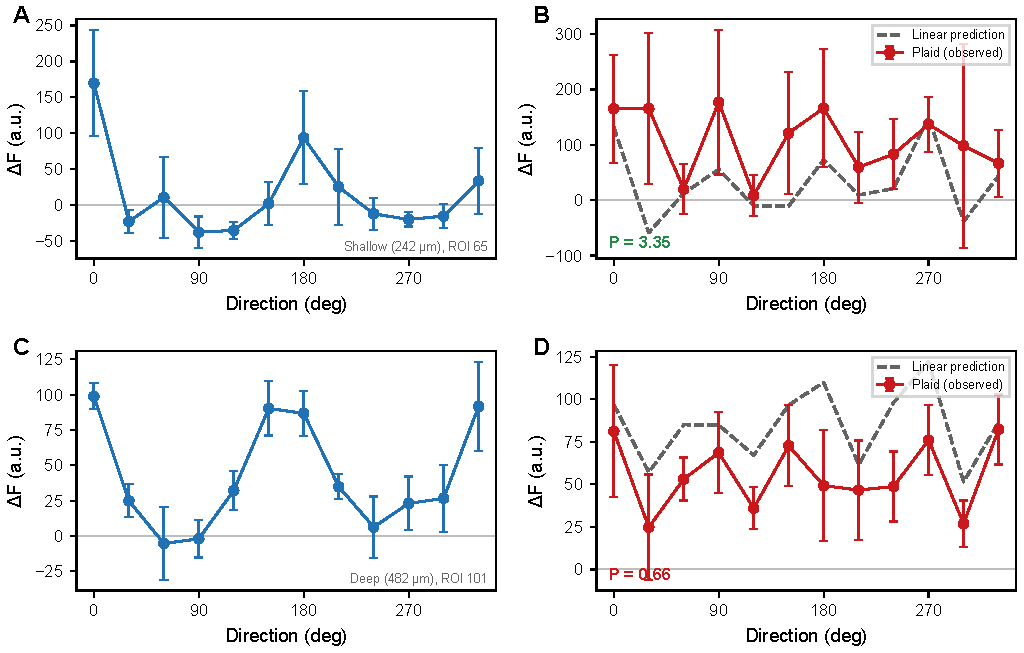
\includegraphics[width=\textwidth]{figures/fig1_tuning_curves.pdf}
  \caption{\textbf{Example cross-orientation analysis at shallow and deep
  cortical depths.}
  \textbf{(A)}~Grating tuning curve ($\Delta F$) for an example ROI at a
  shallow site (242~$\mu$m).
  \textbf{(B)}~Observed plaid response (red) versus linear prediction
  (dashed gray) for the same ROI. $P = 3.35$, indicating strong
  facilitation.
  \textbf{(C)}~Grating tuning curve for an example ROI at a deep site
  (482~$\mu$m).
  \textbf{(D)}~Observed plaid response versus prediction for the deep ROI.
  $P = 0.66$, indicating suppression. Error bars show SEM across trials.}
  \label{fig:stimuli}
\end{figure}

% --- Figure 2: Model schematic ---
\begin{figure}[tbp]
  \centering
  % \includegraphics[width=\textwidth]{figures/fig2_model.pdf}  % TODO: no model figure yet
  \caption{\textbf{Linear prediction model for plaid responses.}
  \textbf{(A)}~Gabor spatial filter at the preferred orientation.
  \textbf{(B)}~Temporal filter modeled as a difference of Maxwell functions
  (time constants $s_1 = 20$~ms, $s_2 = 40$~ms), producing a
  space-time separable linear filter.
  \textbf{(C)}~The linear prediction is the sum of the responses to each
  component grating of the plaid, computed by shifting and summing the
  grating tuning curve. Deviations from this prediction are quantified by
  metrics $P$ (ratio) and $C$ (shape correlation).}
  \label{fig:model}
\end{figure}

\subsection{Cross-orientation suppression increases with cortical depth}

Metric $P$ decreased with cortical depth at the site level ($r = -0.706$,
$p = 2.72 \times 10^{-5}$, $n = 28$; Figure~\ref{fig:depth}A), with
superficial sites (140--266~$\mu$m) exhibiting $P > 1$ (facilitation: the
observed plaid response exceeded the linear prediction) and deeper sites
(392--518~$\mu$m) exhibiting $P < 1$ (suppression). The transition from net
facilitation to net suppression occurred at approximately 350~$\mu$m depth.

% --- Figure 3: P and C vs depth ---
\begin{figure}[tbp]
  \centering
  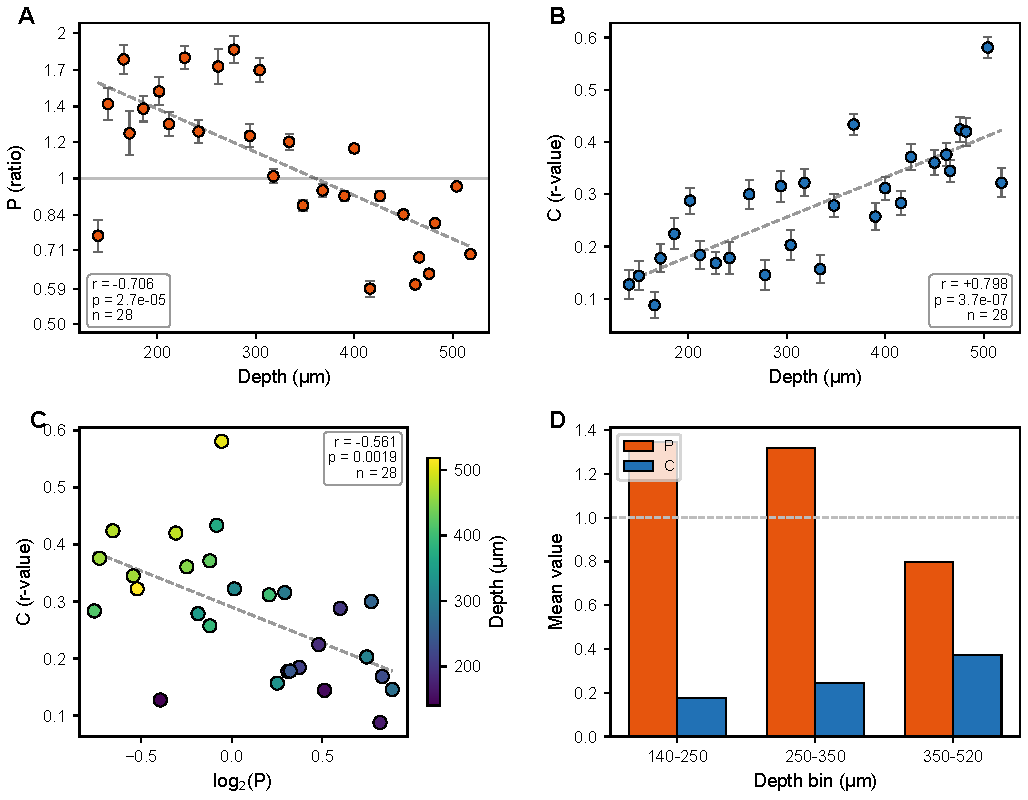
\includegraphics[width=\textwidth]{figures/fig3_depth.pdf}
  \caption{\textbf{Depth-dependent changes in cross-orientation metrics.}
  \textbf{(A)}~Metric $P$ (suppression/facilitation ratio) decreased with
  cortical depth ($r = -0.706$, $p = 2.72 \times 10^{-5}$, $n = 28$). Each
  point represents the site-mean $P$ across all ROIs at one imaging depth,
  plotted on a logarithmic axis. Dashed line shows linear regression.
  $P > 1$: facilitation; $P < 1$: suppression.
  \textbf{(B)}~Metric $C$ (shape similarity) increased with depth
  ($r = +0.799$, $p = 3.38 \times 10^{-7}$). Higher $C$ indicates the plaid
  tuning curve shape is more linearly predictable from grating responses.
  \textbf{(C)}~Scatter plot of $P$ versus $C$ across sites, colored by
  cortical depth, showing their anticorrelation.
  \textbf{(D)}~Depth-binned summary. Superficial layer~2/3 shows facilitation
  ($P > 1$); deep layer~2/3 shows suppression ($P < 1$).}
  \label{fig:depth}
\end{figure}

\subsection{Plaid tuning shape becomes more predictable with depth}

Metric $C$, the Pearson correlation between predicted and observed plaid
tuning curves, increased with depth ($r = +0.799$, 95\% CI:
$[+0.679, +0.892]$, $p = 3.38 \times 10^{-7}$; Figure~\ref{fig:depth}B),
indicating that deeper neurons have plaid tuning curve shapes that are more
linearly predictable from the grating response despite showing stronger
amplitude suppression (lower $P$). The metrics $P$ and $C$ were
anticorrelated across sites ($r = -0.571$, $p = 0.002$;
Figure~\ref{fig:depth}C): as the gain of the plaid response decreased with
depth, its shape became more predictable, consistent with a divisive
normalization mechanism that scales gain while preserving the form of the
tuning curve.

\subsection{Spatial frequency preference varies with depth}

Mean preferred spatial frequency decreased with cortical depth ($r = -0.785$,
$p < 10^{-6}$; Figure~\ref{fig:sf}), consistent with the known laminar
gradient in spatial frequency preference in macaque V1
\citep{devries1982}. Within individual sites, spatial frequency showed weak
correlations with $P$ (significant at 7 of 28 sites), indicating that spatial
frequency preference does not strongly predict $P$ within a single imaging
plane; however, across the full depth range, controlling for spatial frequency
reduced the $P$--depth correlation from $r = -0.706$ to $r = -0.220$
($p = 0.26$), accounting for approximately 69\% of the effect
(Table~\ref{tab:mediation}). This is consistent with a mechanism in which
deeper neurons, preferring lower spatial frequencies, have larger receptive
fields and correspondingly broader normalization pools, producing stronger
cross-orientation suppression.

% --- Figure 4: Spatial frequency ---
\begin{figure}[tbp]
  \centering
  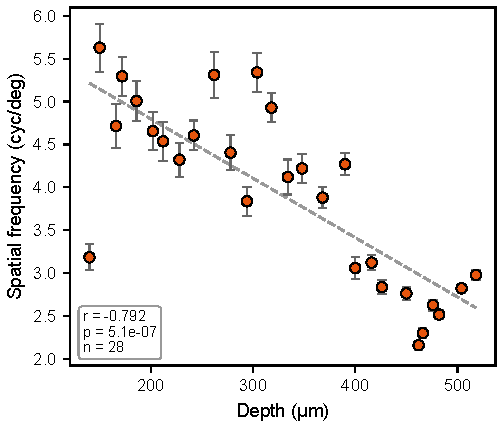
\includegraphics[width=0.5\textwidth]{figures/fig4_sf.pdf}
  \caption{\textbf{Spatial frequency preference decreases with cortical
  depth.} Site-mean preferred spatial frequency plotted against depth. Each
  point is one field of view; error bars show SEM. Dashed line is the
  linear regression fit.}
  \label{fig:sf}
\end{figure}

\subsection{Baseline fluorescence increases with depth}

Baseline fluorescence increased with cortical depth, consistent with the
progressive increase in laser power applied at deeper imaging planes to
compensate for optical scattering (Figure~\ref{fig:baseline}). Within
individual sites, $P$ and baseline fluorescence were uncorrelated at 24 of
28 sites, indicating that the depth gradient in $P$ is not an artifact of
imaging depth. All metrics used baseline-subtracted responses.

% --- Figure 5: Baseline ---
\begin{figure}[tbp]
  \centering
  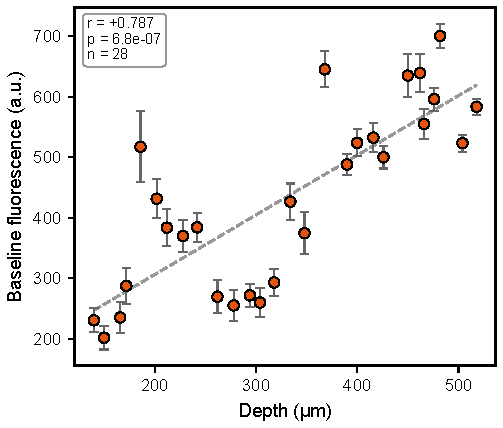
\includegraphics[width=0.5\textwidth]{figures/fig5_baseline.pdf}
  \caption{\textbf{Baseline fluorescence increases with depth.} Site-mean
  baseline fluorescence as a function of cortical depth, reflecting the
  increase in laser power at deeper imaging planes.}
  \label{fig:baseline}
\end{figure}

\subsection{Orientation tuning bandwidth broadens with depth}

Orientation tuning half-width increased with cortical depth ($r = +0.869$,
$p = 2.04 \times 10^{-9}$; Figure~\ref{fig:bandwidth}A), with mean
half-width broadening from approximately $60^{\circ}$ at superficial sites to
approximately $80^{\circ}$ at deeper sites. Within individual sites,
half-width showed a significant negative correlation with $C$ at 15 of 28
sites (Figure~\ref{fig:bandwidth}B): at a given depth, more broadly tuned
neurons tended to have less linearly predictable plaid tuning shapes.
Tuning bandwidth mediated approximately 29\% of the $P$--depth effect
(Table~\ref{tab:mediation}).

% --- Figure 6: Bandwidth ---
\begin{figure}[tbp]
  \centering
  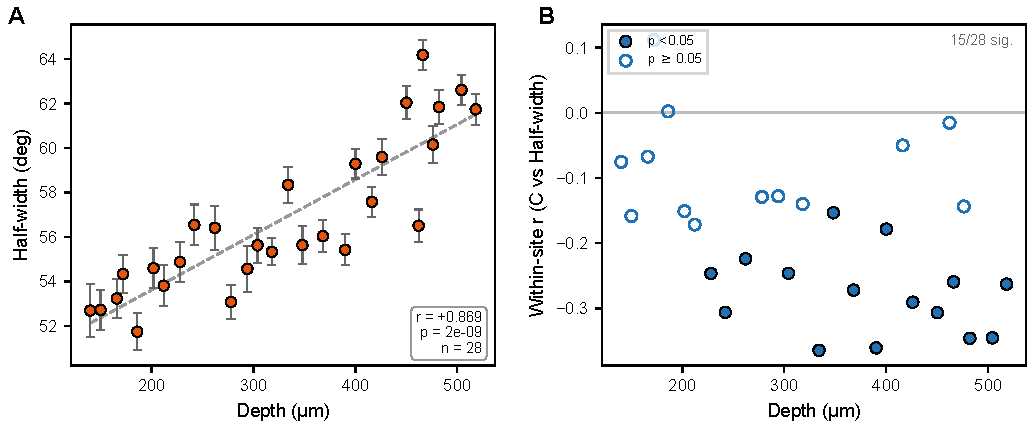
\includegraphics[width=\textwidth]{figures/fig6_bandwidth.pdf}
  \caption{\textbf{Orientation tuning bandwidth increases with depth.}
  \textbf{(A)}~Site-mean half-width at half-height versus depth
  ($r = +0.869$, $p = 2.0 \times 10^{-9}$).
  \textbf{(B)}~Within-site Pearson $r$ between half-width and $C$, plotted
  against depth. Filled circles: $p < 0.05$; open circles: $p \geq 0.05$.
  The consistent negative correlation shows that, within sites, more broadly
  tuned neurons have less predictable plaid tuning shapes.}
  \label{fig:bandwidth}
\end{figure}

\subsection{Local homogeneity decreases with depth}

The local homogeneity index (LHI) showed a strong negative correlation with
depth ($r = -0.93$, $p \ll 0.001$; Figure~\ref{fig:lhi}A), with LHI
decreasing by approximately 35\% from 150 to 520~$\mu$m. This is consistent
with a transition from more homogeneous orientation preference maps in
superficial layer~2/3 (orientation domains) to more heterogeneous maps at
depth (near pinwheel centers or in regions with less columnar organization).

Within individual sites, $C$ and LHI showed a consistently moderate negative
correlation at 26 of 28 sites (Figure~\ref{fig:lhi}B), indicating that
neurons in more heterogeneous orientation neighborhoods (lower LHI, near
pinwheel centers) had more linearly predictable plaid tuning shapes.

% --- Figure 7: LHI ---
\begin{figure}[tbp]
  \centering
  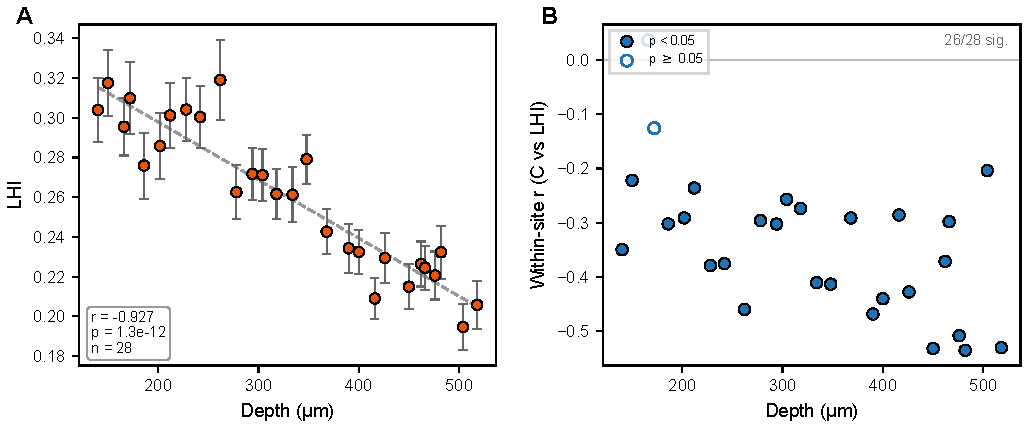
\includegraphics[width=\textwidth]{figures/fig7_lhi.pdf}
  \caption{\textbf{Local homogeneity index decreases with depth.}
  \textbf{(A)}~Site-mean LHI versus depth ($r = -0.93$). Higher LHI
  indicates more homogeneous local orientation preferences (orientation
  domains); lower LHI indicates greater heterogeneity (near pinwheels).
  \textbf{(B)}~Within-site Pearson $r$ between $C$ and LHI, plotted
  against depth. A consistent negative relationship is observed at 26/28
  sites.}
  \label{fig:lhi}
\end{figure}

\subsection{Orientation selectivity decreases with depth}

OSI decreased significantly with cortical depth ($r = -0.490$,
$p = 0.008$; Figure~\ref{fig:osi}A), from approximately 0.70 at
150~$\mu$m to 0.57 at 520~$\mu$m. Within individual sites, $C$ and OSI were
strongly positively correlated at 26 of 28 sites (Figure~\ref{fig:osi}B):
neurons with higher orientation selectivity showed more linearly predictable
plaid tuning. In contrast, $P$ showed a significant within-site relationship
with OSI at only 7 of 28 sites (Figure~\ref{fig:osi}C), suggesting that the
strength of cross-orientation suppression is largely independent of
orientation selectivity within a given imaging plane. Consistent with this,
OSI mediated less than 1\% of the $P$--depth effect in the mediation analysis
(Table~\ref{tab:mediation}).

% --- Figure 8: OSI ---
\begin{figure}[tbp]
  \centering
  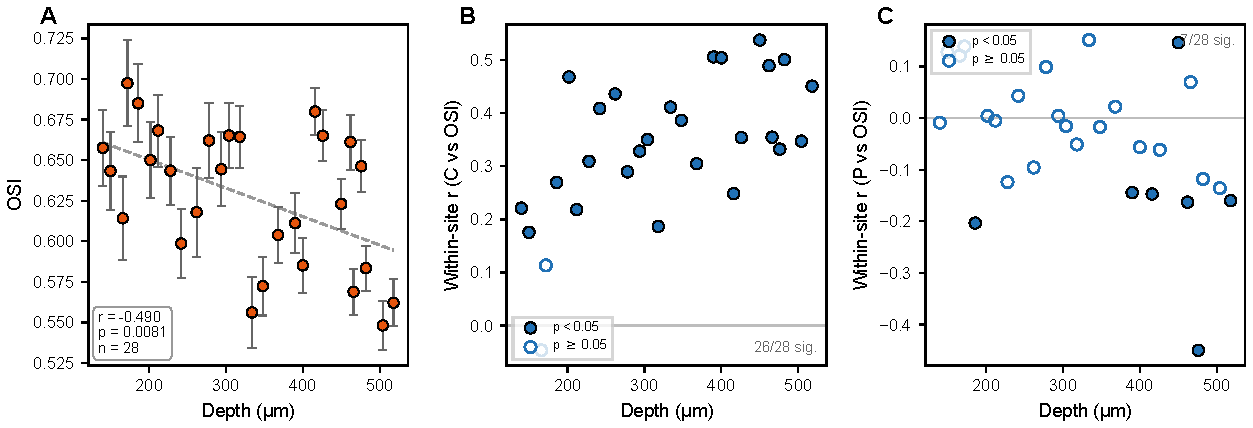
\includegraphics[width=\textwidth]{figures/fig8_osi.pdf}
  \caption{\textbf{Orientation selectivity and cross-orientation metrics.}
  \textbf{(A)}~Site-mean OSI versus depth ($r = -0.490$, $p = 0.008$).
  \textbf{(B)}~Within-site Pearson $r$ between $C$ and OSI versus depth.
  A strong positive relationship is present at 26/28 sites: more
  orientation-selective neurons have more predictable plaid tuning shapes.
  \textbf{(C)}~Within-site Pearson $r$ between $P$ and OSI versus depth.
  Significant at only 7/28 sites.}
  \label{fig:osi}
\end{figure}

\subsection{Robustness and control analyses}

The $P$--depth and $C$--depth correlations remained significant after
controlling for potential confounds using partial correlations
(Table~\ref{tab:controls}). Controlling for ROI radius alone slightly
strengthened the $P$--depth correlation (partial $r = -0.757$,
$p = 3.1 \times 10^{-6}$), indicating that the depth gradient in ROI
morphology does not account for the depth gradient in suppression.
Simultaneous control for ROI radius, SNR, OSI, and spatial frequency
preference reduced the $P$--depth correlation to $r = -0.448$ ($p = 0.017$),
confirming that a significant depth-dependent component of the $P$ gradient
persists beyond all measured confounds. Bootstrap confidence intervals for
the $P$--depth correlation ($r = -0.706$, 95\% CI: $[-0.879, -0.440]$)
excluded zero. The $C$--depth correlation similarly survived all controls
(partial $r = +0.444$, $p = 0.018$).

% --- Table: Mediation ---
\begin{table}[tbp]
  \centering
  \caption{Mediation of the $P$--depth relationship by individual covariates.
    Each row shows the partial correlation between $P$ (log-transformed) and
    depth after controlling for one covariate. Percent reduction is relative
    to the zero-order $r = -0.706$.}
  \label{tab:mediation}
  \begin{tabular}{lcc}
    \toprule
    Control variable & Partial $r$ & \% Reduction \\
    \midrule
    None (zero-order)         & $-0.706$ & ---  \\
    + LHI                     & $-0.173$ & 76\% \\
    + Spatial frequency       & $-0.220$ & 69\% \\
    + Half-width              & $-0.500$ & 29\% \\
    + SNR                     & $-0.682$ &  3\% \\
    + OSI                     & $-0.705$ & $<$1\% \\
    \bottomrule
  \end{tabular}
\end{table}

% --- Table: Partial correlations ---
\begin{table}[tbp]
  \centering
  \caption{Partial correlations between depth and cross-orientation metrics
    after controlling for potential confounds ($n = 28$ sites).}
  \label{tab:controls}
  \begin{tabular}{llcc}
    \toprule
    Metric & Controls & Partial $r$ & $p$-value \\
    \midrule
    $P$ & ROI radius                     & $-0.757$ & $3.1 \times 10^{-6}$ \\
    $P$ & Radius + SNR                   & $-0.765$ & $2.1 \times 10^{-6}$ \\
    $P$ & All (radius + SNR + OSI + SF)  & $-0.448$ & $0.017$ \\
    $C$ & ROI radius                     & $+0.511$ & $0.005$ \\
    $C$ & Radius + SNR                   & $+0.567$ & $0.002$ \\
    $C$ & All (radius + SNR + OSI + SF)  & $+0.444$ & $0.018$ \\
    \bottomrule
  \end{tabular}
\end{table}


\subsection{Summary of depth-dependent changes}

Eight metrics showed coordinated depth-dependent changes across layer~2/3
(Table~\ref{tab:depth_profile}). Superficial layer~2/3 was characterized
by high spatial frequency preference, narrow orientation tuning, high
selectivity, high local homogeneity, and cross-orientation facilitation.
Deeper layer~2/3 showed low spatial frequency preference, broad tuning, lower
selectivity, lower local homogeneity, and cross-orientation suppression.

\begin{table}[tbp]
  \centering
  \caption{Depth profile summary across layer~2/3.}
  \label{tab:depth_profile}
  \begin{tabular}{ll}
    \toprule
    Metric & Change with increasing depth \\
    \midrule
    ROI size (radius, npix)         & Increases  \\
    Baseline fluorescence           & Increases  \\
    SNR                             & Increases  \\
    Orientation tuning bandwidth    & Broader    \\
    Preferred spatial frequency     & Lower      \\
    Orientation selectivity (OSI)   & Lower      \\
    Local homogeneity (LHI)         & Lower      \\
    Cross-orientation ratio ($P$) & More suppressive ($P < 1$) \\
    Shape similarity ($C$)          & More predictable \\
    \bottomrule
  \end{tabular}
\end{table}

% ============================================================================
\section{Discussion}

We found that cross-orientation interactions transition systematically from
facilitation in superficial layer~2/3 to suppression at greater cortical
depth in macaque V1, with the suppression/facilitation ratio $P$ decreasing
significantly with depth ($r = -0.706$, $p = 2.72 \times 10^{-5}$, $n = 28$)
and the shape-similarity metric $C$ increasing ($r = +0.799$,
$p = 3.38 \times 10^{-7}$). The $P$--depth effect was robust to
partial-correlation controls for ROI morphology, signal-to-noise ratio,
orientation selectivity, and spatial frequency preference
($r = -0.448$, $p = 0.017$), and spatial frequency and local orientation
homogeneity each mediated a substantial fraction of the depth gradient.

\subsection{Relation to normalization models}

The observation that $P$ decreases with depth while $C$ increases is
consistent with the divisive normalization framework
\citep{heeger1992, carandini2012}. If deeper neurons draw from broader
normalization pools, the denominator of the normalization equation is larger,
producing stronger divisive suppression (lower $P$) while preserving the
relative shape of the tuning curve (higher $C$). A purely noise-driven
account of the $P$--depth gradient would predict that both $P$ and $C$
degrade together; the observation that they move in opposite directions argues
against this possibility and is instead consistent with a gain-scaling
mechanism that reduces response amplitude while preserving tuning curve form
\citep{carandini1997}.

\subsection{Spatial frequency and tuning bandwidth as mediators}

Controlling for spatial frequency preference reduced the $P$--depth
correlation by 69\%, consistent with the interpretation that deeper neurons,
preferring lower spatial frequencies, have larger receptive fields and
correspondingly broader normalization pools \citep{devries1982, sceniak1999},
which would naturally produce stronger cross-orientation suppression.
Orientation tuning bandwidth mediated 29\% of the effect through a related
mechanism: more broadly tuned neurons at depth are less selective in which
orientations contribute to the normalization pool, again strengthening
suppression. Local orientation homogeneity (LHI) mediated 76\% of the
effect, reflecting the transition from homogeneous orientation domains in
superficial layer~2/3 to more heterogeneous local structure at depth
\citep{nauhaus2008}. Because spatial frequency, bandwidth, and LHI are
themselves intercorrelated and all covary with depth, their individual
mediation percentages overlap substantially. Nevertheless, the combined
partial correlation controlling for radius, SNR, OSI, and SF
($r = -0.448$, $p = 0.017$) confirms that a significant component of the
$P$--depth gradient cannot be accounted for by any of these measured
covariates, suggesting that circuit-level factors---possibly the density or
specificity of inhibitory connections---contribute independently to the
depth gradient in normalization strength.

\subsection{Comparison with prior work}

Nearly all prior characterizations of cross-orientation suppression have
relied on single-unit electrophysiology, recording from one neuron at a
time in cat \citep{morrone1982, bonds1989, deangelis1992} or macaque
\citep{carandini1997, smith2006} V1. These studies established that
suppression is widespread but showed considerable cell-to-cell variability.
Our population-level approach reveals that much of this variability is
structured: it follows a systematic depth gradient across layer~2/3. This
gradient was not accessible to single-electrode studies, which typically
sample isolated neurons without precise depth registration.

Two-photon imaging of cross-orientation suppression has been reported
previously in mouse V1 \citep{busse2009}, but mouse V1 lacks the columnar
organization of primate V1, making direct comparison difficult. The depth
gradient in local orientation homogeneity that we observe---from
high-LHI orientation domains superficially to low-LHI heterogeneous
regions at depth---has no clear analogue in the salt-and-pepper
organization of mouse V1.

\subsection{The $P$--$C$ dissociation}

The anticorrelation between $P$ and $C$ across sites ($r = -0.571$,
$p = 0.002$) provides an important internal control. If the depth gradient in
$P$ were driven by noise, data quality, or neuropil contamination, one would
expect $C$ to decrease in parallel, because noisier data would make tuning
shapes less predictable. Instead, $C$ increases with depth: deeper neurons
have plaid tuning shapes that are more faithfully predicted by the linear
model even as their overall amplitude is reduced. This pattern is difficult to
explain by any artifact of imaging depth and is instead consistent with a
gain-scaling mechanism---divisive normalization---that reduces response
amplitude while preserving the shape of the tuning curve.

\subsection{Limitations}

Several limitations apply. All recordings were obtained from a single animal
(\textit{Macaca nemestrina}); however, the internal consistency of the
$P$--depth gradient across 28 independent fields of view, acquired over
5~recording sessions, provides confidence that the effect is not driven by
idiosyncratic features of a small number of sites. Generalization to other
individuals and species remains to be determined. The design is
correlational: we cannot establish whether the depth gradient in
normalization is caused by the depth gradient in spatial frequency
preference, or whether both are independent consequences of a shared circuit
architecture. ROI radius increases with depth ($r = +0.878$), raising the
concern that larger ROIs at depth average over more neuropil and thus show
artificially lower $P$; however, the $P$--depth partial correlation
controlling for radius strengthens slightly ($r = -0.757$ versus $-0.706$ at
zero order), arguing against this confound. Calcium imaging with GCaMP6s
introduces nonlinearities in the fluorescence-to-activity transformation that
may differ across depth, though these nonlinearities would be expected to
compress response ratios rather than to produce a systematic depth gradient.
Layer boundaries were assigned based on depth from the pial surface without
histological verification, though the depth range (140--518~$\mu$m) is
consistent with the known extent of layer~2/3 in macaque V1
\citep{lund1988}.

\subsection{Future directions}

The tissue from which these recordings were obtained is being prepared for
serial electron microscopy reconstruction \citep{chatterjee2021}. This will
make it possible to compare the physiological properties of thousands of
neurons---including the cross-orientation metrics reported here---with their
reconstructed synaptic connectivity and to test directly whether the residual
depth gradient in $P$ that survives all measured confounds is accounted for by
changes in inhibitory wiring architecture across layer~2/3.

% ============================================================================
\section*{Acknowledgments}

This work was supported by the Allen Institute for Brain Science and the
Department of Neurobiology and Biophysics at the University of Washington.
We thank the staff of the Washington National Primate Research Center for
animal care and surgical support.

% ============================================================================
\bibliography{references}

\end{document}
